\label{ch:typo}

For working with \LaTeX{} you can take advantage of a variety of books and free
introductions and tutorials on the internet.
A competent contact point for \LaTeX{} beginners is the \LaTeX{} Wikibook, which is
available under \url{http://en.wikibooks.org/wiki/LaTeX}. 

The following sections give examples of the most important \LaTeX{} environments
and commands.

\section{Tables}

Tables have to be realized with the help of the \textit{table} environment.
Tables shall be sequentially numbered for each chapter and described in terms
of a short caption (cf.\ \Cref{tab:diplomaseminar}).

\begin{table}[htb]
	\centering
	\begin{tabular}{|l|c|c|}
		\hline \textbf{Name} & \textbf{Date} & \textbf{Title} \\
		\hline
		\hline Mustermann Adam  & 18.5   & T1    \\
		\hline Musterfrau Eva  & 22.6   & T2    \\
		\hline
	\end{tabular}
	\caption{Seminar for Master Students}
	\label{tab:diplomaseminar}
\end{table}


\section{Figures}

Like tables, figures shall be sequentially numbered for each chapter and
described in terms of a short caption.
You could either produce your drawings directly inside \LaTeX{} using
PSTricks, \footnote{\url{http://tug.org/PSTricks}} \pgf/tikz{},
\footnote{\url{http://sourceforge.net/projects/pgf}} or any set of macros
dedicated to your requirements (cf.\ \cref{fig:samplefigure_tikz}).
Alternatively, you may include figures prepared in external tools (cf.\
\cref{fig:samplefigure_pdf}).
Note, to ensure high quality printing, all figures must have at least 300 dpi.


\cfinputfigure{automata}

\begin{figure}[tb]
	\centering
	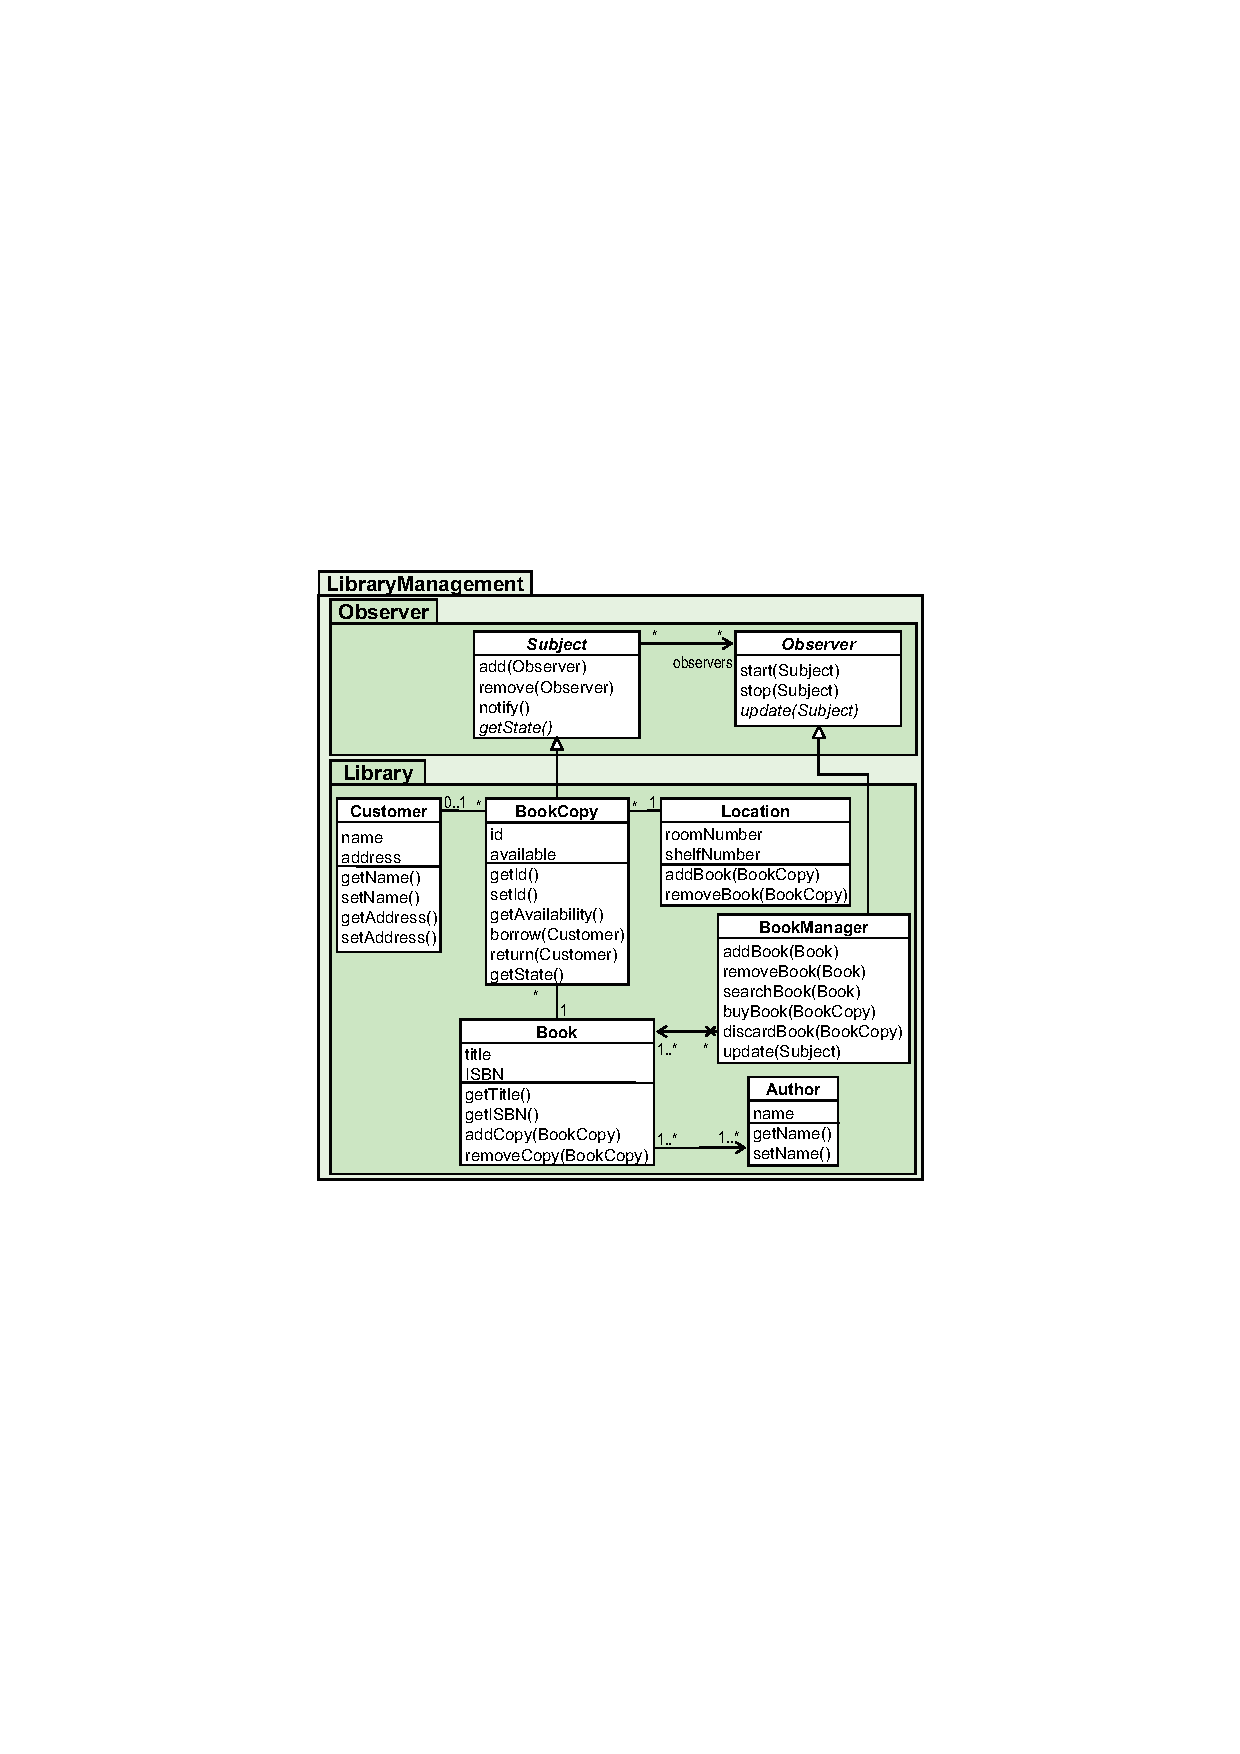
\includegraphics[width=0.7\textwidth]{figures/figure1}
	\caption{Sample figure}
	\label{fig:samplefigure_pdf}
\end{figure}


\section{Fonts}

When introducing important terms for the first time use \emph{emphasize}.
For a consistent look and feel of proper names like \cd and \uml{Observer}
pattern you may define macros in the main document \texttt{thesis.tex}.

\section{Code}

For short code fragments use the \textit{verbatim} environment.

\begin{verbatim}
//Start Program
System.out.println("Hello World!");
//End Program
\end{verbatim}

A much better alternative is the \textit{algorithm} environment (cf.\
\cref{alg:samplealgorithm}).
This environment offers special formatting features for loops, operations and
comments.

\cfinputalgorithms{samplealgorithm}
